\documentclass[12pt,a4paper]{article}
\usepackage{fontspec}
\usepackage{polyglossia}
\setdefaultlanguage{russian}
\setmainfont{STIX Two Text}[AutoFakeBold=1.5]
\setmonofont{Menlo}
\newfontfamily\cyrillicfonttt{Menlo}
\usepackage[a4paper,margin=2cm]{geometry}
\usepackage{graphicx,longtable,tabularx,array,booktabs}
\usepackage{float,caption,enumitem,pdflscape,xurl,listings,tikz}
\usepackage{hyperref,etoolbox}
\usetikzlibrary{positioning}
\hypersetup{colorlinks=true,linkcolor=blue,urlcolor=blue}
\lstset{basicstyle=\ttfamily\footnotesize,breaklines=true,columns=fullflexible,frame=single,keepspaces=true,showstringspaces=false}
\setlength{\parindent}{1.25cm}
\setlength{\parskip}{0.25em}
\renewcommand{\arraystretch}{1.16}
\setlist{nosep,leftmargin=1.5em}
\AtBeginEnvironment{longtable}{\small}
\sloppy
\begin{document}
\begin{titlepage}
\centering
{\large Практическая работа\par}
\vspace{2.5cm}
{\LARGE\bfseries Отчёт по практической работе № 5\par}
\vspace{0.6cm}
{\Large Безопасная обработка пользовательского ввода\par}
\vspace{1.8cm}
\begin{tabular}{p{4cm}p{11cm}}
Дисциплина: & Основы разработки защищённого программного обеспечения и компьютерных сетей\\
Вариант: & 19 — Система учёта транспортных средств организации\\
Исходная версия: & v0.4\\
Версия работы: & v0.5 — Secure Input Validation\\
Студент: & Мостовая Полина Андреевна\\
Группа: & ИУСбд-02-23
\end{tabular}
\vfill
{\large 2026\par}
\end{titlepage}
\tableofcontents
\clearpage
\section{Тема и цель работы}
Цель работы — разработать и проверить централизованную безопасную проверку входных данных до передачи в бизнес-логику. Реализация продолжает проект v0.4 и сохраняет предметные валидаторы транспортных средств.

\section{Индивидуальный вариант и проект}
Вариант 19 требует нового логического типа вложения. Добавлен точный allowlist-ключ \texttt{vehicle\_photo} для обозначения фотографии транспортного средства. Это идентификатор типа, а не путь и не имя файла. Загрузка и хранение изображений не входят в реализацию.

\section{Спецификация валидации}
Вход — UTF-8 JSON bytes размером не более 8192 байт. Обязательные поля: \texttt{title} (5–100 символов), \texttt{description} (20–2000), \texttt{category} (network/software/access/other), \texttt{priority} (строгое целое 1–5). Необязательны \texttt{reporter\_ip} (IPv4/IPv6/null) и \texttt{attachment\_key} (log/screenshot/report/vehicle\_photo/null). Неизвестные и повторные ключи запрещены. Текст нормализуется NFC, внешние пробелы удаляются; CRLF описания нормализуется в LF. Управляющие символы запрещены, кроме перевода строки в описании.

HTML-подобный ввод сохраняется как текст. При выводе в HTML требуется отдельное контекстное экранирование. NFC объединяет канонически эквивалентное представление, но не подменяет символы по совместимости, как NFKC.

\section{Схема обработки сообщения}
Схема \texttt{docs/input\_validation\_flow.mmd} показывает получение bytes, лимит размера, UTF-8, JSON-разбор, структуру, нормализацию и allowlist. Отказы на каждом этапе безопасны. TB-01 — существующая граница между недоверенным вводом и приложением; проверенная модель передаётся дальше только после всех проверок.
\begin{figure}[H]
\centering
\begin{tikzpicture}[node distance=7mm,box/.style={draw,rounded corners,align=center,text width=10cm,minimum height=8mm,font=\small},arrow/.style={->,thick}]
\node[box] (a) {Получение JSON bytes};
\node[box,below=of a] (b) {Проверка размера: не более 8192 байт};
\node[box,below=of b] (c) {Строгая UTF-8 декодировка и разбор JSON};
\node[box,below=of c] (d) {Проверка структуры, повторов и неизвестных полей};
\node[box,below=of d] (e) {NFC, trim, CRLF; типы, длины, диапазоны и allowlist};
\node[box,below=of e] (f) {Неизменяемый ValidatedRequest};
\node[box,below=of f] (g) {Сервисный уровень};
\foreach \x/\y in {a/b,b/c,c/d,d/e,e/f,f/g} {\draw[arrow] (\x) -- (\y);}
\node[draw,fill=gray!12,align=center,text width=4cm,below left=2mm and 2cm of c,font=\small] (x) {Безопасный отказ\\без исходных данных};
\foreach \n in {b,c,d,e} {\draw[arrow,dashed] (\n.west) -- (x.east);}
\draw[red,densely dashed,thick] ([xshift=-1.2cm]a.north west) -- ([xshift=-1.2cm]g.south west);
\node[rotate=90,fill=white,font=\small] at ([xshift=-1.2cm]e.west) {TB-01};
\end{tikzpicture}
\caption{Проверка на доверительной границе TB-01 до передачи модели дальше}
\end{figure}

\section{Реализация}
Центральный модуль возвращает неизменяемую типизированную модель. CLI ограничивает чтение до 8193 байт и отдаёт короткий JSON-ответ без исходного содержимого и traceback.
\subsection{Модель и обработка сообщения}
\lstinputlisting[language=Python]{../../app/validation.py}
\subsection{CLI}
\lstinputlisting[language=Python]{../../app/input_cli.py}

\section{Таблица тестовых сценариев}
Каждая строка соответствует сценариям раздела 10.1 задания. Фактический результат записан по запуску pytest после реализации; таблица будет дополнена реальными скриншотами на следующем этапе.
\small
\begin{longtable}{p{0.7cm}p{6.3cm}p{2.4cm}p{3cm}p{1.9cm}}
\caption{Обязательные сценарии и фактические результаты}\\
\toprule № & Проверка & Ожидание & Фактический результат & Статус\\\midrule\endfirsthead
\toprule № & Проверка & Ожидание & Фактический результат & Статус\\\midrule\endhead
1 & Корректное обращение & Принято & Тест пройден & Пройдено\\
2 & Отсутствует обязательное поле & Отказ & Тест пройден & Пройдено\\
3 & Неизвестное поле & Отказ & Тест пройден & Пройдено\\
4 & Короткий заголовок & Отказ & Тест пройден & Пройдено\\
5 & Слишком длинное описание & Отказ & Тест пройден & Пройдено\\
6 & Неизвестная категория & Отказ & Тест пройден & Пройдено\\
7 & Приоритет меньше 1 & Отказ & Тест пройден & Пройдено\\
8 & Приоритет больше 5 & Отказ & Тест пройден & Пройдено\\
9 & Приоритет-строка & Отказ & Тест пройден & Пройдено\\
10 & Приоритет True & Отказ & Тест пройден & Пройдено\\
11 & Некорректный IP & Отказ & Тест пройден & Пройдено\\
12 & Неизвестное вложение & Отказ & Тест пройден & Пройдено\\
13 & Путь вместо ключа & Отказ & Тест пройден & Пройдено\\
14 & Повреждённый JSON & Отказ & Тест пройден & Пройдено\\
15 & Размер более 8192 байт & Отказ & Тест пройден & Пройдено\\
16 & Повторяющиеся ключи & Отказ & Тест пройден & Пройдено\\
17 & Управляющий символ & Отказ & Тест пройден & Пройдено\\
18 & Корректный IPv6 & Принято & Тест пройден & Пройдено\\
19 & Канонически эквивалентный Unicode & NFC & Тест пройден & Пройдено\\
20 & HTML-подобный текст & Сохранён как текст & Тест пройден & Пройдено\\
\bottomrule
\end{longtable}
\normalsize

\subsection{Дополнительные проверки варианта 19}
\small
\begin{longtable}{p{5cm}p{3cm}p{4.7cm}p{1.9cm}}
\toprule Сценарий & Ожидание & Фактический результат & Статус\\\midrule
vehicle\_photo & Принято & Тест пройден & Пройдено\\
Неизвестный тип & Отказ & Тест пройден & Пройдено\\
Имя файла vehicle\_photo.jpg & Отказ & Тест пройден & Пройдено\\
\bottomrule
\end{longtable}
\normalsize

\section{Фактические проверки}
Первичный системный \texttt{python3} оказался устаревшим и не поддерживает синтаксис проекта. Проверки выполнены штатным окружением проекта \texttt{./.venv/bin/python -m pytest -q}: получено 92 passed; ошибок и пропусков нет. Реальный CLI принял два корректных файла с кодом 0 и отклонил два некорректных с кодом 2. В коде \texttt{app/} нет вызовов системных команд. В тестах \texttt{subprocess.run} запускает CLI с постоянными аргументами, без shell, а пользовательские данные передаются через stdin. Результаты команд показаны на рисунках~\ref{fig:cli}–\ref{fig:review}.

\begin{figure}[H]
\centering
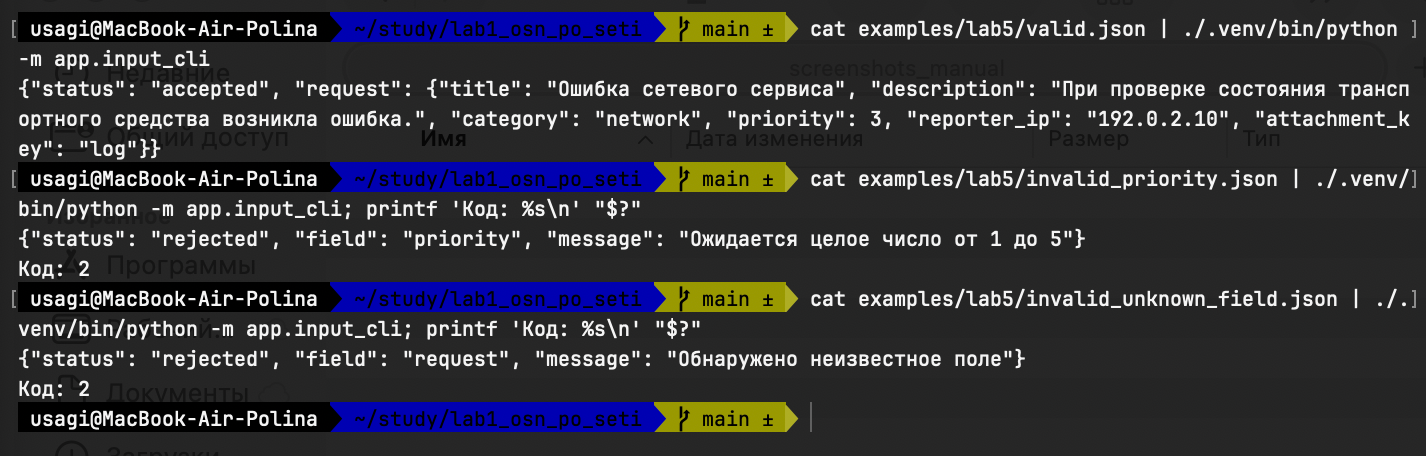
\includegraphics[width=0.96\textwidth,height=0.42\textheight,keepaspectratio]{screenshots_manual/lab5_1and2.png}
\caption{Принятие корректного обращения и контролируемый отказ по приоритету и неизвестному полю.}
\label{fig:cli}
\end{figure}
\begin{figure}[H]
\centering
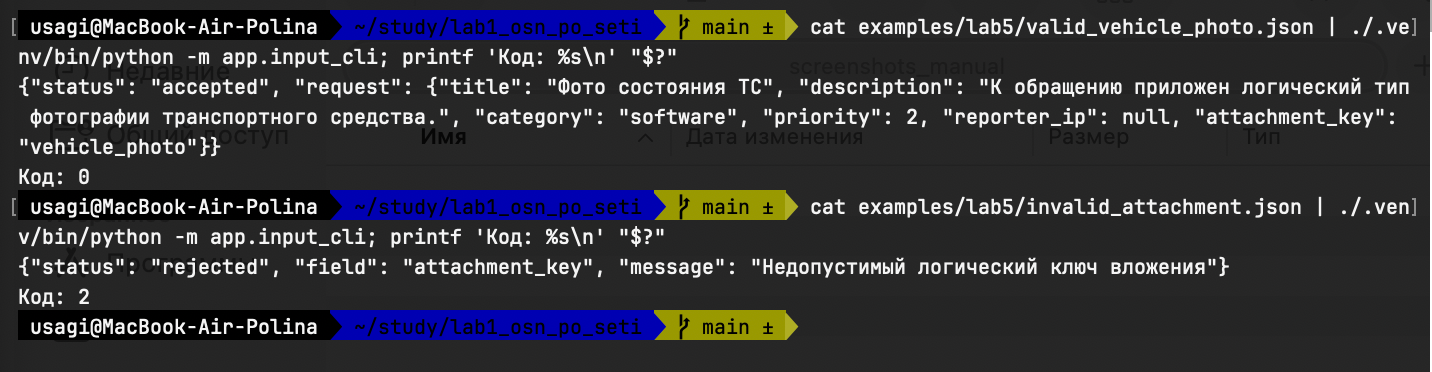
\includegraphics[width=0.96\textwidth,height=0.42\textheight,keepaspectratio]{screenshots_manual/lab5_3.png}
\caption{Проверка логического ключа \texttt{vehicle\_photo} и отклонение пути вместо ключа.}
\label{fig:variant}
\end{figure}
\begin{figure}[H]
\centering
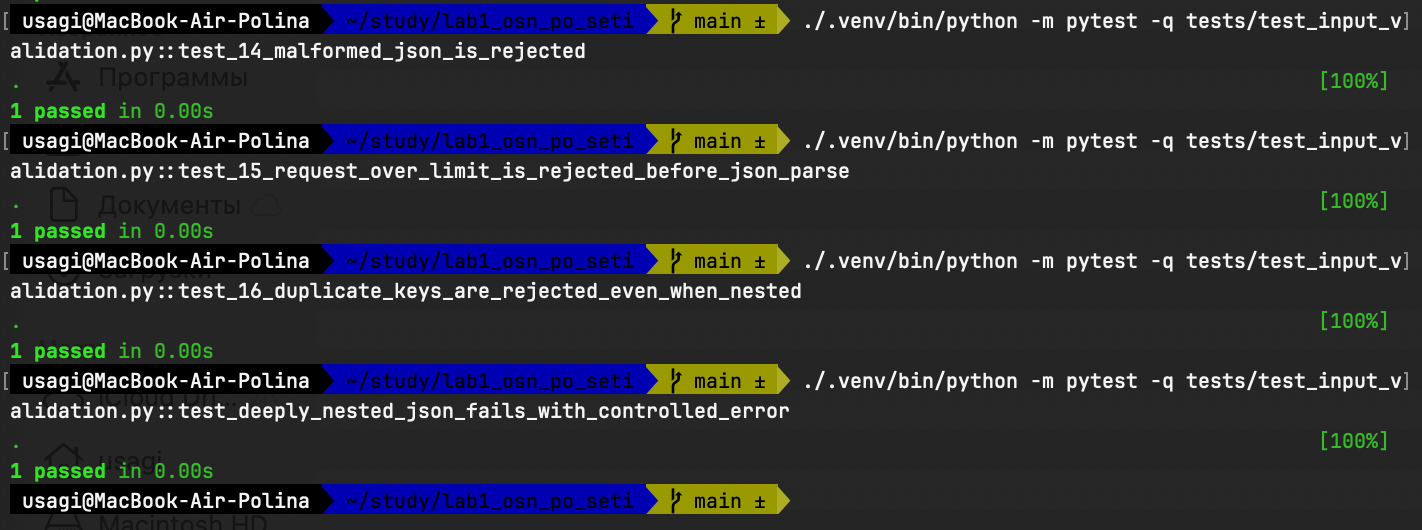
\includegraphics[width=0.96\textwidth,height=0.42\textheight,keepaspectratio]{screenshots_manual/lab5_4.png}
\caption{Негативные проверки JSON, размера сообщения, дублирования ключей и глубокой вложенности.}
\label{fig:parser}
\end{figure}
\begin{figure}[H]
\centering
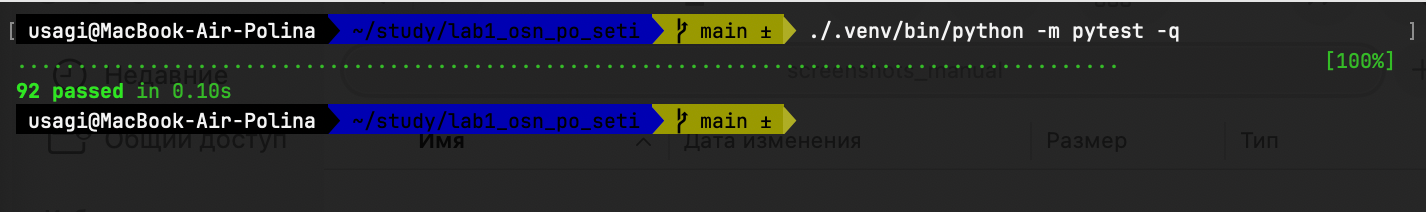
\includegraphics[width=0.96\textwidth,height=0.42\textheight,keepaspectratio]{screenshots_manual/lab5_5.png}
\caption{Полный запуск автоматизированного набора: 92 теста пройдены.}
\label{fig:tests}
\end{figure}
\begin{figure}[H]
\centering
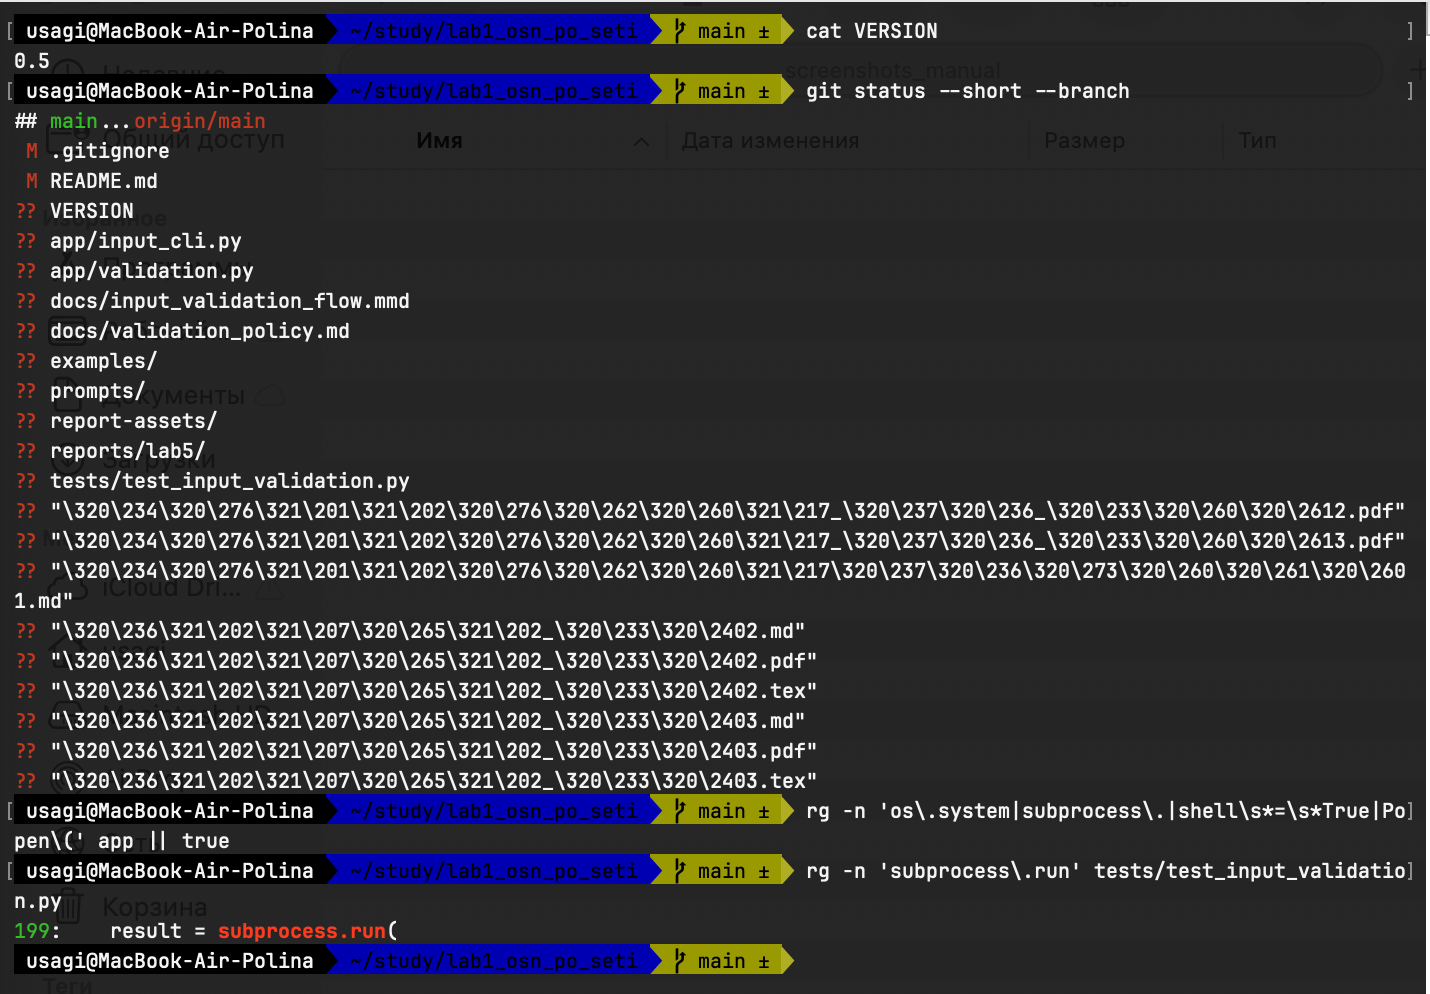
\includegraphics[width=0.96\textwidth,height=0.42\textheight,keepaspectratio]{screenshots_manual/lab5_6.png}
\caption{Версия проекта, состояние рабочей копии и поиск вызовов команд ОС.}
\label{fig:review}
\end{figure}

\section{Обнаруженные и исправленные ошибки}
Первый сбор тестов выявил два несвязанных вопроса: системный python3 не соответствовал версии Python проекта, а вспомогательная проверка отсутствия утечки некорректно сравнивала пустую строку. Использован проектный virtualenv и исправлено тестовое утверждение. После этого добавлены проверки граничных значений, глубокой вложенности и фактической CLI-точки. Ошибок реализации после повторной проверки не осталось; причины уязвимого поведения в исходном проекте этим тестированием не устанавливались.

\section{Анализ Path Traversal и Command Injection}
Пользовательское значение вложения проверяется сравнением с фиксированным allowlist и не используется в файловых операциях. В приложении не найдено \texttt{os.system}, \texttt{subprocess}, \texttt{Popen} или \texttt{shell=True}. В тесте интеграции безопасный \texttt{subprocess.run} запускает CLI с постоянными аргументами и без оболочки. Модуль не запускает системные команды.

\section{Соответствие требованиям}
\begin{longtable}{p{5cm}p{5cm}p{4cm}}
\toprule Требование & Реализация & Проверка\\\midrule
Лимит и UTF-8 & До JSON-разбора & Негативные тесты\\
JSON-структура и дубликаты & Строгий parser hook & Негативные тесты\\
Типы и диапазоны & \texttt{ValidatedRequest} & 20 обязательных сценариев\\
Вариант 19 & \texttt{vehicle\_photo} & Три отдельных теста\\
Защита от path traversal & Ключ не является путём & Отказ пути/имени файла\\
Безопасная диагностика & Только имя поля и общий текст & Проверка отсутствия эха\\
\bottomrule
\end{longtable}

\section{Ограничения прототипа}
CLI локальный и не является сетевым API; аутентификация, авторизация для заявок, база данных, файловое хранилище и загрузка изображения не реализованы. Лимит размера не ограничивает частоту запросов. Валидация не заменяет SQL-параметризацию или контекстное экранирование вывода.

\section{Ответы на контрольные вопросы}
\begin{enumerate}
\item Проверка устанавливает, соответствует ли вход контракту до его использования.
\item Проверяет доверенная сторона, потому что клиентские проверки можно обойти или изменить.
\item Синтаксическая проверка проверяет форму; семантическая — допустимый смысл и диапазон.
\item NFC помогает привести канонически одинаковые Unicode-строки к одному представлению.
\item Каноническое представление — согласованная форма значения для сравнения и обработки.
\item Строки являются данными; допустимость определяется контекстом и контрактом, а не поиском подозрительных подстрок.
\item Allowlist перечисляет допустимое; denylist перечисляет известное недопустимое и может пропускать новые варианты.
\item Ограничение поля не учитывает общий размер JSON, структуру и служебные накладные расходы.
\item В Python \texttt{bool} — подкласс \texttt{int}, поэтому используется проверка точного типа.
\item \texttt{ipaddress.ip\_address()} проверяет IPv4/IPv6 и строит объект адреса.
\item Неизвестное поле может незаметно менять смысл операции или обходить предположения слоя приложения.
\item Разные JSON-парсеры могут выбрать разные значения дублирующегося ключа.
\item Путь из пользовательских данных может выйти за пределы разрешённого каталога.
\item Path Traversal — использование сегментов пути для обращения к файлу вне разрешённой области.
\item \texttt{shell=True} интерпретирует строку оболочкой и может превратить данные в команды.
\item Проверка входа не гарантирует безопасную сборку SQL; запросы следует параметризовать.
\item Валидация решает, допустимо ли значение; HTML-экранирование безопасно представляет его в конкретном контексте.
\item HTML-подобная строка может быть обычным текстом; удаление меняет данные и не заменяет безопасный вывод.
\item Негативное тестирование проверяет ожидаемый отказ на ошибочных и намеренно некорректных входах.
\item Fail Secure — при сбое отказать безопасно, не продолжая частично операцию.
\item Собственный тип ошибки позволяет отличать отказ контракта и безопасно формировать ответ.
\item Не раскрывают исходный запрос, секреты, внутренние пути и трассировку исключения.
\item Клиентскую проверку можно обойти; доверенный сервер проверяет заново.
\item Разделение данных и команд обеспечивают параметризация запросов, фиксированные аргументы и отказ от оболочки.
\item Соответствие показывают трассируемая политика, тесты ожидаемого результата и проверяемые фактические выводы.
\end{enumerate}

\section{Вывод}
Создан отдельный валидатор JSON и CLI, сохраняющие прежнюю предметную валидацию автопарка. Контракт формирует неизменяемую модель, а вариант 19 расширяет список логических типов вложений ключом \texttt{vehicle\_photo}. Тесты подтверждают только проверенные свойства прототипа; они не доказывают безопасность будущего веб-интерфейса или файлового хранилища.

\section{Источники}
\begin{enumerate}
\item Практическая работа №5 «Безопасная обработка пользовательского ввода», предоставленная методичка, 2026.
\item Документы проекта v0.2–v0.4: требования, модель угроз, реестр рисков и защищённая архитектура.
\item Python 3: стандартные модули \texttt{json}, \texttt{unicodedata}, \texttt{ipaddress}.
\end{enumerate}
\end{document}
